\documentclass[a4paper, twoside, openright, 11pt, oldfontcommands]{memoir}
\usepackage[T1]{fontenc}
\usepackage{microtype}
\OnehalfSpacing
\usepackage{cite}
\usepackage{amsmath}
\usepackage{amssymb}
\usepackage{hyperref}
\hypersetup{
    colorlinks,
    citecolor=black,
    filecolor=black,
    linkcolor=black,
    urlcolor=black
}
\usepackage[authoryear,square]{natbib}
\usepackage{bibentry}
\renewcommand{\cite}{\citep}

%%% Formatting setup
% 11pt Palatino (URW Palladio) for text
\renewcommand{\rmdefault}{ppl}
% Optima (URW Classico) for headings
%\renewcommand{\sfdefault}{uop}

% Use Courier which has a bold series
\renewcommand{\ttdefault}{pcr}

% Make our pretty chapter headings
% Copied from DaveC via Adam
\usepackage[bf,sf]{titlesec}
\newcommand{\chapformat}[1]{\parbox[c]{0.8\textwidth}{\Huge #1}}
\titleformat{\chapter}[hang]
    {\sffamily\bfseries}
    {\parbox[c]{0.2\textwidth}{\rmfamily\fontsize{72}{72}
     \selectfont\thechapter\hspace{10pt}\rule[-12pt]{2pt}{72pt}}}
    {0pt}
    {\chapformat}

\title{Addressing the Performance Bottlenecks of Device Driver Synthesis}

\author{Alexander Legg \\
    \\
    Supervised by \\
Leonid Ryzhyk, Nina Narodytska, and Gernot Heiser}

\begin{document}

\maketitle

\setcounter{secnumdepth}{3}
\setcounter{tocdepth}{3}
\tableofcontents

\begin{abstract}

Device drivers are notorious for their contribution to the failure of software
systems. A driver forms the interface between two complicated systems: an
operating system and a hardware device. As a result, driver development is
complicated and highly prone to human error. Driver reliability has been the
focus of much research over the past two decades. One result of this research
is device driver synthesis.

Device driver synthesis aims to remove human error from the development process
by removing humans. A synthesis tool can take a formal specification of
requirements and produce a system. Thus, a driver can be synthesised by
providing the tool with a specification of the OS and the hardware that it must
interface with. The resulting driver is guaranteed to be correct with respect
to the specifications.

The drawback of this approach is that synthesis is a computationally intensive
task belonging to 2-EXPTIME. In practice synthesis tools are capable of
producing drivers though there remain cases where synthesis is impossible. In
this thesis I will present an algorithm that provides results on many of these
previously unattainable cases.

\end{abstract}

\renewcommand{\abstractname}{Acknowledgements}
\begin{abstract}
Acknowledge some people
\end{abstract}

\chapter{Introduction}

We rely on software systems to perform important tasks for us on a daily basis. Unfortunately we also frequently experience the frustration of an incorrect software system. However, as these systems become more ingrained into our lives the cost of incorrectness can be far greater than mere frustration.

In 1996 the European Space Agency lost their Ariane 5 rocket forty seconds after launch to an incorrect conversion from floating point to integer~\cite{Dowson97}. The cost of the failure was \$370 million in USD. More recently, Toyota has been forced to recall a large number of vehicles due to a failure in the software controlling the brakes~\cite{Parrish13}. The failures led to loss of life~\cite{CBS10}.

As the desire for software and the consequences of incorrectness has grown, the need for a systematic methodology for producing correct software has become apparent. One solution has been to develop strict engineering practices, including rigorous testing, to reduce the chance of errors. Another solution is to produce a proof of correctness of the software, either with or without the aid of a mechanised proof assistant. Model checking can also be used in some cases to automate the correctness proof.

A step further is to have our software automatically constructed for us, a technique first formally considered by Alonzo Church in the middle of the last century~\cite{Church62}. Software synthesis shifts the role of the developer from writing code to writing formal specifications. This completely eradicates the human error factor from the low level construction of software and allows developers to focus on high level system design. In all other approaches to software correctness the software must first be constructed; a process involving considerable time and effort.

Unfortunately, automatic software synthesis involves nontrivial computation. In broad strokes, the synthesis algorithm must determine how the state of the system is affected by the software and its environment and then select actions for the software such that no matter the actions of the environment the system adheres to the specification. In practice, on certain system specifications the process can lead to significant \emph{state explosion} that renders synthesis infeasible.

The state of the art in synthesis contains several methodologies that act as countermeasures to state explosion. However, no single approach is suited to all classes of specifications nor are all specifications currently feasible. In this thesis I propose a methodology for resisting state explosion on a set of synthesis specifications that are problematic for other approaches.

\section{Synthesis}

This thesis is concerned with synthesis of reactive systems. In a reactive system a controller interacts \emph{continuously} with its environment by responding to inputs with the appropriate outputs. For example, a device driver is a reactive system in which the driver interacts with an operating system and a hardware device. Synthesising reactive systems like drivers is different to synthesising regular programs or functions since the correctness of a controller depends on how the system behaves over time instead of a single output corresponding to a single input. As a result, the reactive synthesis problem is staged as a game between the controller and its environment. For a detailed formalisation see Chapter~\ref{ch:background}.

This thesis is concerned with synthesis of controllers for safety games in which the winning condition for the controller is defined by ensuring that the game remains within a set of safe states. The game is zero sum, the environment wins if a state outside the safe set is reached. We say that we have \emph{solved} a game if we can construct a winning strategy for one of the players. The usual approach to solving safety games is to iteratively construct a set of winning states that are known to be safe regardless of the actions of the environment. A winning strategy for the controller can be constructed by choosing actions that have successor states within the winning region.

Explicit enumeration of the states in the winning region is infeasible even on small specifications so the set of states is usually represented symbolically. This is done by specifying the game with states as valuations of a set of boolean variables and using boolean algebra to symbolically define sets of states. Traditionally binary decision diagrams (BDDs) are used to represent boolean functions because they provide compact representations in most cases and there are efficient algorithms for operating on formulas in BDD form. The disadvantage of this approach is that in the worst case the representation occupies space that is exponential in the number of variables in the formula. A BDD is a canonical representation of a formula so it may be the case that a compact BDD representing the winning region for a particular specification does not exist.

Other approaches rely on satisfiability solvers to efficiently perform the operations required by synthesis on sets of states. The satisfiability problem (SAT) is the question of whether a value can be assigned to all variables in a formula such that the formula evaluates to true. Modern SAT solvers provide efficient implementations of backtracking search with computational learning that operate on boolean formulas in clausal normal form (CNF). The advantage of a SAT based approach is that CNF is not canonical so in cases when a BDD cannot compactly represent a set of states it may be possible to do so in CNF.

The disadvantage of SAT based approaches is that solvers only determine whether a satisfying assignment to variables \emph{exists}. This is known as existential quantification. The dual problem, universal quantification, is to determine whether all variable assignments satisfy a formula. Both forms of quantification are required for synthesis in order to decide whether an action exists for one player that satisfies a property for all opponent actions. An example of this kind of computation would be deciding whether the controller can force the game into the winning region regardless of any action the environment chooses. It is possible to perform universal quantification with a SAT solver but it adds considerable complexity, which introduces another bottleneck to the synthesis process.

\section{Approach}

This thesis presents a SAT based approach that computes an approximation of the winning region. By approximating the winning region we hope to avoid the state explosion cost of representing the entire set of winning states. The algorithm is set within a counterexample guided abstraction refinement framework. This is our approach to handling the alternating quantifications of synthesis. Candidate strategies are constructed and refined via counterexamples instead of precisely computing the result of the quantified formula.

In this approach, a SAT solver is used to verify whether a candidate strategy is a winning strategy for a safety game with a fixed number of a game rounds, which we call a bounded game. This approach is similar to bounded model checking where a program is verified by querying a SAT solver for a trace that violates the specification. In our bounded synthesis approach the SAT solver searches for a trace of opponent moves that cause the candidate strategy to lose the bounded game. As with bounded model checking, a counterexample trace informs the algorithm how to refine the candidate strategy.

Discovering a winning strategy for the bounded game does not guarantee that the strategy is winning in the unbounded game. Specifically, if the controller strategy avoids an error state for $k$ rounds the SAT solver cannot guarantee that it can avoid errors for $k+1$ rounds. We address this problem with an extension to the algorithm that iteratively solves bounded games while incrementing the bound. During the execution of the bounded game solver we learn losing states for both players. This computational learning serves a dual purpose by both serving as an optimisation to reduce the search space and also providing the termination condition. By carefully learning states that are losing for the environment we may construct an overapproximation of the environment's winning region. The overapproximation can be used to guarantee that the actual winning region does not contain the initial states and so there cannot be a winning strategy for the environment.


\section{Contribution}

This thesis presents a SAT based counterexample guided approach to controller synthesis of safety specifications. This approach includes a bounded synthesis algorithm, an extension to unbounded synthesis, and a methodology for extracting strategies from the certificate generated by the bounded synthesis algorithm. 

The approach is designed to solve synthesis specifications where the winning region is difficult to represent compactly with existing symbolic techniques. The aim of this work was not to produce a one size fits all approach to safety synthesis but instead to provide a solution suited to problem instances that are difficult to solve for other methods.

The instances that emit winning regions that are difficult to efficiently represent with binary decision diagrams include many real world problems. An example of such a specification is an arbiter that must grant resources from a homogeneous pool in order to fulfil requests from the environment. In this problem the winning region for the environment must exclude all combinations of resource allocations that exceed the number of requests. There is no compact representation of this kind of winning region as a binary decision diagram but in our approach we use overapproximation so that we don't need to find and represent all combinations.

In order to validate the methodology I have implemented the algorithm as an open source tool. In later chapters we present benchmarks that show that the algorithm is promising and although it does not solve as many problem instances as other techniques it performs better on certain classes of problems.


\section{Summary}

\begin{itemize}

    \item \emph{Reactive synthesis} can be used to automatically generate correct-by-construction controllers for software systems. Compared to other approaches to software correctness synthesis does not require the software to first be developed.

    \item Synthesis is formalised as a game between a controller and its environment. In many cases these games can be solved by constructing a symbolic representation of the winning states of the game using a binary decision diagram. However, for some games there is no compact representation of the winning region.

    \item This thesis presents a SAT based counterexample guided approach that targets these cases by constructing an approximation of the winning region that is sufficient to determine the winner of the game.

\end{itemize}


%%%\section{Device Drivers}

%%%Device drivers are the software that allows the operating system to interface
%%%with hardware. The role of the driver is to manipulate the inputs of the device
%%%so that it remains in a error-free state and correctly handles the requests of
%%%the operating system. By way of example consider an ethernet driver. The driver
%%%accepts requests to send and receive data packets from the OS and acts on those
%%%requests by reading from and writing to buffers on the device. It must ensure
%%%that those buffers are maintained in a usable state by correctly updating a
%%%register containing the location of the head of the buffer queue.

%%%According to a study performed in 2011~\cite{Palix11}, drivers account for
%%%approximately 57\% of the lines of code in the Linux kernel and subsequently is
%%%the largest source of bugs. The study also analysed the staging directory of
%%%the kernel, which contains all in-progress drivers, and found it to contain the
%%%highest fault rate (faults per line of code) out of any directory in the
%%%kernel. The results of the study give evidence to the widely held belief that
%%%correct drivers are hard to produce.

%%%Consequences of buggy drivers

%%%This thesis focuses on automatic construction of correct drivers as a solution
%%%to the driver problem. Alternate approaches, of which there are many, will be
%%%discussed in Chapter~\ref{ch:relatedwork}.



\chapter{Background}

This is the background.


\chapter{Related Work}
\label{ch:relatedwork}

\chapter{Bounded Realisability}
\label{ch:bounded}

\newtheorem*{exmp}{Example}
\newtheorem*{exmpI}{Example: Intuition behind the algorithm}

In this chapter I will describe my work on bounded realisability of reactive systems with safety properties. As introduced in Chapter~\ref{ch:background} reactive realisability is the problem of determining the existence of a program, which we call a \emph{controller}, that continuously interacts with its environment in adherence with a specification. A safety property is a simple correctness condition that lays out a set of states of the system that controller must stay within. In this chapter we will refer to this property in the negation: the controller must avoid \emph{error states}.

Realisability is the first step on the path to synthesis. In the subsequent chapter I will describe an algorithm that extracts the actions of the controller necessary for realisation. This strategy may be used for synthesis: automatic construction of the controller program. Reactive synthesis for controllers with safety properties has many practical uses in areas such as circuit design, device drivers, or industrial automation.

The algorithm described in this chapter solves bounded safety games. Recall that Chapter~\ref{ch:background} introduced games as a formalism for synthesis. In this chapter we are concerned with \emph{bounded} games that restrict all runs to certain length. This concept is borrowed from model checking where it is used for similar aims. Specifically, runs of a bounded game can be checked by a purely propositional formula passed to a SAT solver. The SAT solver provides an efficient method for quickly discovering counterexamples. The algorithm presented here is a counterexample guided abstraction refinement framework that relies on counterexamples to find and refine player strategies.

The primary motivation of this work is to avoid computing the entire set of winning states as would be done in the standard controllable predecessor driven fixpoint algorithm. An explicit representation of the winning set would quickly run into the state explosion issues of synthesis so traditionally the set is represented symbolically with a binary decision diagram. However, a BDD is a canonical representation of a set that, in the worst case, may be exponential in the number of variables. For some systems there is no compact representation of the winning set and for those cases an algorithm that does not compute it, such as the one presented here, is desirable.

\section{Inspiration}

This work draws inspiration from a QBF solving algorithm that treats the QBF problem as a game~\cite{Janota12}. In that algorithm one player assumes the role of the universal quantifiers and the opponent takes on the existential quantifiers. In the game, the players take turns to chooses values for their variables from the outermost quantifier block in. One method of solving QBF games is to expand the formula for each quantified variable by either conjuncting (for universal quantification) or disjuncting (for existential) the formula with the variable set to each possible value. For large QBF instances this expanded formula becomes far too large to solve so the authors introduce abstractions, or partially expanded formulas, to avoid expanding on variables unnecessarily. The abstractions are refined through a CEGAR process of searching for candidate solutions and analysing counterexamples. The full algorithm is described in detail in Chapter~\ref{ch:related}. The bounded synthesis algorithm presented here takes inspiration from the CEGAR framework of this work and can be thought of as a domain specific version of the QBF algorithm.

\section{Algorithm}

\begin{exmp}

We introduce a running example to assist the explanation. We consider a simple
arbiter system in which the environment makes a request for a number of
resources (1 or 2), and the controller may grant access to up to two resources.
The total number of requests grows each round by the number of environment
requests and shrinks by the number of resources granted by the controller in
the previous round.  The controller must ensure that the number of unhandled
requests does not accumulate to more than 2.  Figure~\ref{fig:example} shows
the variables (\ref{fig:examplevars}), the initial state of the system (\ref{fig:exampleinit}), 
and the formulas for computing next-state
variable assignments (\ref{fig:exampletrans}) for this example. We use primed identifiers
to denote next-state variables and curly braces to define the domain of a
variable.

This example is the $n=2$ instance of the more general problem of an arbiter of
$n$ resources. For large values of $n$, the set of winning states has no compact representation, which
makes the problem hard for BDD solvers. In Section~3 we will outline how the
unbounded game can be solved without enumerating all winning states.

\end{exmp}

\begin{figure}
    \begin{subfigure}[t]{\textwidth}
        \centering
        \begin{tabular}{l | l | l}
            \textbf{Controllable} & \textbf{Uncontrollable} & \textbf{State} \\
            \hline
            \texttt{request : \{1, 2\}} & \texttt{grant0 = \{0, 1\}} & \texttt{resource0 = \{0, 1\}} \\
            & \texttt{grant1 : \{0, 1\}} & \texttt{resource1 = \{0, 1\}} \\
            & & \texttt{nrequests : \{0, 1, 2, 3\}} \\
        \end{tabular}
        \caption{Variables}
        \label{fig:examplevars}
    \end{subfigure}

    \begin{subfigure}[t]{\textwidth}
        \centering
        \texttt{resource0 = 0; resource1 = 0; nrequests = 0;}
        \caption{Initial State}
        \label{fig:exampleinit}
    \end{subfigure}

    \begin{subfigure}[t]{\textwidth}
        \begin {align*}
            \texttt{resource0'} & \texttt{ = grant0;} \\
            \texttt{resource1'} & \texttt{ = grant1;} \\
            \texttt{nrequests'} & \texttt{ = (nrequests + request >= resource0 + resource1)} \\ 
                                & \texttt{ ? (nrequests + request - resource0 - resource1) : 0;}
        \end{align*}
        \caption{Transition Relation}
        \label{fig:exampletrans}
    \end{subfigure}
    \caption{Example}
    \label{fig:example}
\end{figure}

Our bounded synthesis algorithm constructs abstractions of the game 
that restrict actions available to one of the players.
Specifically, we consider abstractions represented as trees of actions,
referred to as \emph{abstract game trees} (AGTs).  Figure~\ref{fig:agt} shows
an example abstract game tree restricting the environment (abstract game trees
restricting the controller are similar).  In the abstract game, the controller
can freely choose actions whilst the environment is required to pick actions
from the tree.  After reaching a leaf, the environment continues playing
unrestricted.  The tree in Figure~\ref{fig:agt} restricts the first environment
action to \texttt{request=1}. At the leaf of the tree the game continues
unrestricted.

The root of the tree is annotated by the initial state $s$ of the abstract game
and the bound $k$ on the number of rounds.  We denote $\textsc{nodes}(T)$ the
set of all nodes of a tree $T$, $\textsc{leaves}(T)$ the subset of leaf nodes.
For edge $e$, $\textsc{action}(e)$ is the action that labels the edge, and for
node $n$, $\textsc{height}(k, n)$ is the distance from n to the last round of a
game bounded to $k$ rounds.  $\textsc{height}(k, T)$ is the height of the root
node of the tree.  For node $n$ of the tree, $\textsc{succ}(n)$ is the set of
pairs $\langle e, n' \rangle$ where $n'$ is a child node of $n$ and $e$ is the
edge connecting $n$ and $n'$.

\tikzset{every node/.style={solid}}
\tikzstyle{fixed}=[solid]
\begin{figure}
    \centering
    \captionsetup[subfigure]{width=\textwidth,justification=raggedleft}
    \begin{subfigure}[t]{.2\textwidth}
        \centering
        \begin{minipage}[t][3.8cm][t]{\textwidth}
        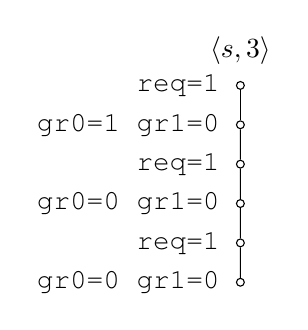
\begin{tikzpicture}[level distance = 5mm,baseline]
            \node [circle,draw,inner sep=1pt] (root){}
                child {node [circle,draw,inner sep=1pt] {}
                    child {node [circle,draw,inner sep=1pt] {}
                        child {node [circle,draw,inner sep=1pt] {}
                            child {node [circle,draw,inner sep=1pt] {}
                                child {node [circle,draw,inner sep=1pt] {}
                                    node [left=4pt] {\texttt{gr0=0 gr1=0}}
                                }
                                node [left=4pt] {\texttt{req=1}}
                            }
                            node [left=4pt] {\texttt{gr0=0 gr1=0}}
                        }
                        node [left=4pt] {\texttt{req=1}}
                    }
                node [left=4pt] {\texttt{gr0=1 gr1=0}}
                }
                node [left=4pt] {\texttt{req=1}}
                node [above=4pt] {$\langle s, 3 \rangle$};
        \end{tikzpicture}
    \end{minipage}
        \caption{Controller winning trace}
        \label{fig:trace}
    \end{subfigure}
    \begin{subfigure}[t]{.2\textwidth}
        \centering
        \begin{minipage}[t][3.8cm][t]{\textwidth}
        \begin{tikzpicture}[dash pattern = on 2pt off 2pt, level distance = 10mm,baseline]
            \node [circle,draw] (root){}
                child {node [circle,draw] {}
                    edge from parent [fixed] node [left] {\texttt{gr0=1 gr1=0}}
                }
                node [left=4pt] {}
                node [above=4pt] {$\langle s, 3 \rangle$};
        \end{tikzpicture}
        \end{minipage}
        \caption{AGT}
        \label{fig:agt}
    \end{subfigure}
    \begin{subfigure}[t]{.2\textwidth}
        \centering
        \begin{minipage}[t][3.8cm][t]{\textwidth}
        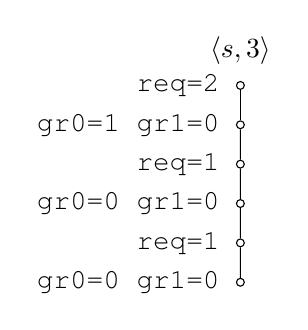
\begin{tikzpicture}[level distance = 5mm,baseline]
            \node [circle,draw,inner sep=1pt] (root){}
                child {node [circle,draw,inner sep=1pt] {}
                    child {node [circle,draw,inner sep=1pt] {}
                        child {node [circle,draw,inner sep=1pt] {}
                            child {node [circle,draw,inner sep=1pt] {}
                                child {node [circle,draw,inner sep=1pt] {}
                                    node [left=4pt] {\texttt{gr0=0 gr1=0}}
                                }
                                node [left=4pt] {\texttt{req=1}}
                            }
                            node [left=4pt] {\texttt{gr0=0 gr1=0}}
                        }
                        node [left=4pt] {\texttt{req=1}}
                    }
                node [left=4pt] {\texttt{gr0=1 gr1=0}}
                }
                node [left=4pt] {\texttt{req=2}}
                node [above=4pt] {$\langle s, 3 \rangle$};
        \end{tikzpicture}
        \end{minipage}
        \caption{Environment winning trace}
        \label{fig:trace2}
    \end{subfigure}
    \begin{subfigure}[t]{.2\textwidth}
        \centering
        \begin{minipage}[t][3.8cm][t]{\textwidth}
        \begin{tikzpicture}[dash pattern = on 2pt off 2pt, level distance = 10mm,baseline]
            \node [circle,draw] (root){}
                child {node [circle,draw] {}
                    edge from parent [fixed] node [left] {\texttt{gr0=1 gr1=0}}
                }
                node [left=4pt] {\texttt{req=2}}
                node [above=4pt] {$\langle s, 3 \rangle$};
        \end{tikzpicture}
        \end{minipage}
        \caption{Partial Strategy}
        \label{fig:strategy}
    \end{subfigure}
    \caption{Abstract game trees.}
    \label{fig:alltrees}
\end{figure}


Given an environment (controller) abstract game tree $T$ a \emph{partial
strategy} $Strat: \textsc{nodes}(T) \rightarrow \mathcal{C}$ ($Strat: \textsc{nodes}(T)
\rightarrow \mathcal{U}$) labels each node of the tree with the controller's
(environment's) action to be played in that node.   Given a partial strategy
$Strat$, we can map each leaf $l$ of the abstract game tree to $\langle
s',i'\rangle=\textsc{outcome}(\langle s, i\rangle, Strat, l)$ obtained by
playing all controllable and uncontrollable actions on the path from the root
to the leaf.  An environment (controller) partial strategy is \emph{winning against $T$} 
if all its outcomes are states that are winning for the environment (controller)
in the concrete game.


%%%Figure~\ref{fig:strategy} shows an example partial strategy for
%%%the controller.  The controller responds to the requests by first granting
%%%access to \texttt{resource1}, then to \texttt{resource0} in the second round.

\begin{exmpI}

    %% Make it clear that this is intuition only
    We present the intuition behind our bounded synthesis method by applying
    its \emph{simplified version} to the running example.  We begin by finding
    a trace of length $k$ (here we consider $k=3$) that is winning for the
    controller, i.e., that starts from the initial state and avoids the error
    set for three game rounds (see Figure~\ref{fig:trace}).  We use a SAT
    solver to find such a trace, precisely as one would do in bounded model
    checking.  Given this trace we make an initial conjecture that any trace
    starting with action \texttt{gr0=1 gr1=0} is winning for the controller.
    This conjecture is captured in the abstract game tree shown in
    Figure~\ref{fig:agt}.  We validate this conjecture by searching for a
    counterexample trace that reaches an error state with the first controller
    action fixed to \texttt{gr0=1 gr1=0}.   Such a trace, that refutes the
    conjecture, is shown in Figure~\ref{fig:trace2}.  In this trace, the
    environment wins by playing \texttt{req=2} in the first round.  This move
    represents the environment's partial strategy against the abstract game
    tree in Figure~\ref{fig:agt}.  This partial strategy is shown in
    Figure~\ref{fig:strategy}.
    
    Next we strengthen the abstract game tree taking this partial strategy into account.
    To this end we again use a SAT solver to find a trace where the contoller
    wins while the environment plays according to the partial strategy.  In the
    resulting trace (Figure~\ref{fig:trace3}), the controller plays \texttt{gr0=1 gr1=1} in
    the second round.  We refine the abstract game tree using this move as
    shown in Figure~\ref{fig:refined1}.  The environment's partial strategy was
    to make two requests in the first round, to which the controller responds
    by now granting an additional two resources in the second round.

    When the controller cannot refine the tree by extending existing branches,
    it backtracks and creates new branches. Eventually, we obtain the abstract
    game tree shown in Figure~\ref{fig:refined2} for which there does not exist
    a winning partial strategy on behalf of the environment.  We conclude that
    the bounded game is winning for the controller.

\end{exmpI}

\begin{figure}
    \centering
    \begin{subfigure}[t]{.2\textwidth}
        \centering
        \begin{minipage}[t][3.8cm][t]{\textwidth}
        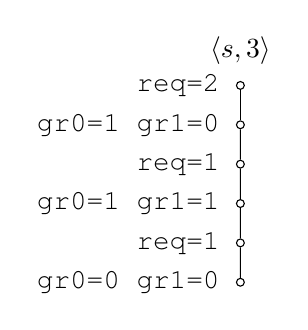
\begin{tikzpicture}[level distance = 5mm,baseline]
            \node [circle,draw,inner sep=1pt] (root){}
                child {node [circle,draw,inner sep=1pt] {}
                    child {node [circle,draw,inner sep=1pt] {}
                        child {node [circle,draw,inner sep=1pt] {}
                            child {node [circle,draw,inner sep=1pt] {}
                                child {node [circle,draw,inner sep=1pt] {}
                                    node [left=4pt] {\texttt{gr0=0 gr1=0}}
                                }
                                node [left=4pt] {\texttt{req=1}}
                            }
                            node [left=4pt] {\texttt{gr0=1 gr1=1}}
                        }
                        node [left=4pt] {\texttt{req=1}}
                    }
                node [left=4pt] {\texttt{gr0=1 gr1=0}}
                }
                node [left=4pt] {\texttt{req=2}}
                node [above=4pt] {$\langle s, 3 \rangle$};
        \end{tikzpicture}
        \end{minipage}
        \caption{Controller winning trace}
        \label{fig:trace3}
    \end{subfigure}
    \begin{subfigure}[t]{.3\textwidth}
        \centering
        \begin{minipage}[t][3.8cm][t]{\textwidth}
        \hspace*{0.8cm}
        \begin{tikzpicture}[dash pattern = on 2pt off 2pt, level distance = 10mm,baseline]
            \node [circle,draw] (root){}
                child {node [circle,draw] {}
                    child {node [circle,draw] {}
                        edge from parent [fixed] node [left] {\texttt{gr0=1 gr1=1}}
                    }
                    edge from parent [fixed] node [left] {\texttt{gr0=1 gr1=0}}
                }
                node [above=4pt] {$\langle s, 3 \rangle$};
        \end{tikzpicture}
        \end{minipage}
        \caption{First refined AGT}
        \label{fig:refined1}
    \end{subfigure}
    \begin{subfigure}[t]{.4\textwidth}
        \centering
        \begin{minipage}[t][3.8cm][t]{\textwidth}
        \begin{tikzpicture}[dash pattern = on 2pt off 2pt, level distance = 10mm,baseline]
            \node [circle,draw] (root){}
                child {node [circle,draw] {}
                    child {node [circle,draw] {}
                        child {node [circle,draw] {}
                            edge from parent [fixed] node [left] {\texttt{gr0=1 gr1=1}}
                        }
                        edge from parent [fixed] node [left] {\texttt{gr0=1 gr1=1}}
                    }
                    edge from parent [fixed] node [left] {\texttt{gr0=1 gr1=0}}
                }
                child {node [circle,draw] {}
                    child {node [circle,draw] {}
                        child {node [circle,draw] {}
                            edge from parent [fixed] node [right] {\texttt{gr0=1 gr1=1}}
                        }
                        edge from parent [fixed] node [right] {\texttt{gr0=1 gr1=1}}
                    }
                    edge from parent [fixed] node [right] {\texttt{gr0=1 gr1=1}}
                }
                node [above=4pt] {$\langle s, 3 \rangle$};
        \end{tikzpicture}
        \end{minipage}
        \caption{Final Refined AGT}
        \label{fig:refined2}
    \end{subfigure}
    \caption{Refined abstract game trees.}
    \label{fig:refinedtrees}
\end{figure}


\begin{algorithm}[t]
    \begin{algorithmic}[1]
        \Function{solveAbstract}{$p, s, k, T$}
        \State $cand \gets $ \Call{findCandidate}{$p, s, k, T$} \Comment{Look for a candidate}
        \IIf{$k = 1$} \Return $cand$ \EndIIf \Comment{Reached the bound}
        \State $T' \gets T$
        \Loop
            \IIf{$cand = \texttt{NULL}$} \Return $\texttt{NULL}$ \EndIIf \Comment{No candidate: return with no solution}
            \State $\langle cex, l, u \rangle \gets $ \Call{verify}{$p, s, k, T, cand$} \Comment{Verify candidate}
            \IIf{$cex = \False$} \Return $cand$ \EndIIf \Comment{No counterexample: return candidate}
            \State $T' \gets $ \Call{append}{$T', l, u$} \Comment{Refine $T'$ with counterexample}
            \State $cand \gets $ \Call{solveAbstract}{$p, s, k, T'$} \Comment{Solve refined game tree}
        \EndLoop
        \EndFunction
        \algstore{b1}
    \end{algorithmic}

    \begin{algorithmic}
        \algrestore{b1}
        \Function{findCandidate}{$p, s, k, T$}
        \State $\hat{T} \gets $ \Call{extend}{$T$} \Comment{Extend the tree with unfixed actions}
            \State $f \gets $ \IfElse{$p = \texttt{cont}$}{\Call{treeFormula}{$k, \hat{T}$}}{\Call{\textoverline{treeFormula}}{$k, \hat{T}$}} \EndIfElse
            \State $sol \gets $ \Call{SAT}{$s(X_{\hat{T}}) \land f$}
            \If{$sol = \texttt{unsat}$} 
                \If{\texttt{unbounded}} \Comment{Active only in the unbounded solver}
                    %\State $\sigma \gets $ \Call{generalise}{$s$} \Comment{Expand $s$ to a set of states}
                    \State \IfElse{$p = \texttt{cont}$}{\Call{learn}{$s, \hat{T}$}}{\Call{\textoverline{learn}}{$s, \hat{T}$}} \EndIfElse
                \EndIf
                \State \Return $\texttt{NULL}$ \Comment{No candidate exists}
            \Else
                \State \Return $\{ \langle n, c \rangle | n \in $ \Call{nodes}{$T$} $, c = \Call{sol}{n} \}$ \Comment{Fix candidate moves in $T$}
            \EndIf
        \EndFunction
        \algstore{b2}
    \end{algorithmic}

    \begin{algorithmic}
        \algrestore{b2}
        \Function{verify}{$p, s, k, T, cand$}
            \For{$l \in leaves(gt)$}
            \State $\langle k', s'\rangle \gets $ \Call{outcome}{$s, k, cand, l$} \Comment{Get bound and state at leaf}
                \State $u \gets $ \Call{solveAbstract}{\Call{opponent}{$p$}, $s'$, $k'$, $\emptyset$} \Comment{Solve for the opponent}
                \IIf{$u \neq \texttt{NULL}$} \Return $\langle \True, l, u \rangle$ \EndIIf \Comment{Return counterexample}
            \EndFor
            \State \Return $\langle \False, \emptyset, \emptyset \rangle$
        \EndFunction
    \end{algorithmic}

    \caption{Bounded synthesis}
    \label{alg:bounded}
\end{algorithm}

The full bounded synthesis algorithm is more complicated: upon finding a candidate 
partial strategy on behalf of player $p$ against abstract game tree $T$, it first checks whether the strategy is winning 
against $T$.  By only considering such strong candidates, we reduce the number of 
refinements needed to solve the game.  To this end, the algorithm checks whether each 
outcome of the candidate strategy is a winning state for $\textsc{opponent}(p)$ by recursively 
invoking the synthesis algorithm on behalf of the opponent.  Thus, our bounded
synthesis algorithm can be seen as running two competing solvers, for the
controller and for the environment. 

%The solvers build candidate partial strategy 
%for their corresponding players, which are used to refine the abstractions.


The full procedure is illustrated in Algorithm~\ref{alg:bounded}.  The
algorithm takes a concrete game $G$ with maximum bound $\kappa$ as an implicit
argument.  In addition, it takes a player $p$ (controller or environment),
state $s$, bound $k$ and an abstract game tree $T$ and returns a winning
partial strategy for $p$, if one exists.  The initial invocation of the
algorithm takes the initial state $I$, bound $\kappa$ and an empty abstract
game tree $\emptyset$.  Initially the solver is playing on behalf of the
environment since that player takes the first move in every game round.  The
empty game tree does not constrain opponent moves, hence solving such an
abstraction is equivalent to solving the original concrete game.

The algorithm is organised as a counterexample-guided abstraction refinement
(CEGAR) loop.  The first step of the algorithm uses the \textsc{findCandidate}
function, described below, to come up with a candidate partial strategy that is
winning when the opponent is restricted to $T$.  If it fails to find a
strategy, this means that no winning partial strategy exists against the opponent
playing according to $T$.  If, on the other hand, a
candidate partial strategy is found, we need to verify if it is indeed winning
for the abstract game $T$.

The \textsc{verify} procedure searches for a \emph{spoiling} counterexample
strategy in each leaf of the candidate partial strategy by calling
\textsc{solveAbstract} for the opponent. The dual solver solves games on behalf
of the opponent player.  

If the dual solver can find no spoiling strategy at any of the leaves, then the
candidate partial strategy is a winning one. Otherwise, \textsc{verify} returns
the move used by the opponent to defeat a leaf of the partial strategy, which
is appended to the corresponding node in $T$ in order to refine it in line~(9).

We solve the refined game by recursively invoking \textsc{solveAbstract} on it.
If no partial winning strategy is found for the refined game then there is also
no partial winning strategy for the original abstract game, and the algorithm
returns a failure.  Otherwise, the partial strategy for the refined game is
\emph{projected} on the original abstract game by removing the leaves
introduced by refinements. The resulting partial strategy becomes a candidate
strategy to be verified at the next iteration of the loop. In the worst case
the loop terminates after all actions in the game are refined into the abstract
game.

The CEGAR loop depends on the ability to guess candidate partial strategies in
\textsc{findCandidate}. For this purpose we use the heuristic that a partial
strategy may be winning if each \textsc{outcome} of the strategy can be
extended to a run of the game that is winning for the current player.  Clearly,
if such a partial strategy does not exist then no winning partial strategy can
exist for the abstract game tree. We can formulate this heuristic as a SAT
query, which is constructed recursively by $\textsc{treeFormula}$ (for the
controller) or $\textsc{\textoverline{treeFormula}}$ (for the environment) in
Algorithm~\ref{alg:treeFormula}.

The tree is first extended to the maximum bound with edges that are labeled
with arbitrary opponent actions (Algorithm~\ref{alg:bounded}, line 14).  For
each node in the tree, new SAT variables are introduced corresponding to the
state ($X_T$) and action ($U_T$ or $C_T$) variables of that node. Additional
variables for the opponent actions in the edges of $T$ are introduced ($U_e$ or
$C_e$) and set to $\textsc{action}(e)$.  The state and action variables of node
$n$ are connected to successor nodes $\textsc{succ}(n)$ by an encoding of the
transition relation and constrained to the winning condition of the player.

%%%Then copies of state and action variables are introduced for each node in the
%%%tree and opponent action variables for each edge $e$ are set to
%%%$\textsc{action}(e)$. 

%%%Candidates are discovered by passing a formulation of the abstract game tree to
%%%a SAT solver in $\textsc{findCandidate}$. This formula contains CNF encodings
%%%of all of the unrolled runs represented by the tree and the winning condition
%%%of the current player.  Runs are encoded by copying the transition relation for
%%%every step in the abstract game. When playing for the controller, the SAT
%%%solver searches for a satisfying assignment to the unfixed label variables in
%%%tree so that none of the runs reaches the error state. The environment
%%%formulation is satisfiable if any run does reach the error state.  The formula
%%%is constructed recursively from the root of a tree by $\textsc{treeFormula}$
%%%(see Algorithm~\ref{alg:treeFormula}).

%%%Since the game tree formulation is passed to a SAT solver, both controllable
%%%and uncontrollable unfixed labels will be existentially quantified. This means
%%%that the SAT solver will find any way to win the game while both players are
%%%cooperating. If no winning run exists in an abstract game even when the players
%%%are cooperating then there is no winning run when the opponent is playing
%%%adversarily. When a winning run is found, the actions chosen by the SAT solver
%%%are used to refine the game tree. This is advantageous for many synthesis
%%%problems where the game must be formalised as adversarial for correctness but
%%%the final implementation will cooperate with its environment in the real world.
%%%An example of such a system is a device driver that cooperates with the device
%%%and OS to provide the interface between the two.

\begin{algorithm}
    \caption{Tree formulas for Controller and Environment respectively}
    \label{alg:treeFormula}
    \begin{algorithmic}[1]
        \Function{treeFormula}{$k, T$}
        \If{$\Call{height}{k, T} = 0$}
        \State \Return{ $\lnot \Call{E}{X_{T}}$ }
        \Else
        \State \Return{$\lnot \Call{E}{X_{T}} \land$ \\
            $$\bigwedge_{\langle e, n \rangle \in \Call{succ}{T}}(\Call{$\delta$}{X_T, U_e, C_T, X_n} \land U_e = \Call{action}{e} \land \Call{treeFormula}{k, n})$$
        }
        \EndIf
        \EndFunction
        \algstore{tf1}
    \end{algorithmic}

    \begin{algorithmic}[1]
        \algrestore{tf1}
        \Function{\textoverline{treeFormula}}{$k, T$}
        \If{$\Call{height}{k, T} = 0$}
        \State \Return{\Call{E}{$X_{T}$}}
        \Else
        \State \Return{ $\Call{E}{X_{T}} \lor$ \\
        $$\bigvee_{\langle e, n \rangle \in \Call{succ}{T}}(\Call{$\delta$}{X_T, U_T, C_e, X_n} \land C_e = \Call{action}{e} \land \Call{\textoverline{treeFormula}}{k, n})$$ }
        \EndIf
        \EndFunction
    \end{algorithmic}
\end{algorithm}

\section{Optimisations}

In this section we present several optimisations to the algorithm.

\subsection{Bad State Learning}

The most important optimisation that allows the algorithm to avoid much of the search space is to record states that are known to be losing for one player. On subsequent calls to the SAT solver we encode these states in the candidate strategy formula (see Algorithm~\ref{alg:treeFormulaLearning}). Thus the algorithm avoids choosing moves that lead to states that are already known to be losing.

Bad states are learned from failed attempts to find a candidate. If the SAT solver cannot find a candidate strategy for a given abstract game tree that means that there is a fixed prefix in the game tree for which the current player can never win. The state reached by playing the moves in the prefix must then be a losing state with some caveats. If the state is at the node with height $k$ and losing for the environment then we know that the environment cannot force to the error set in $k$ rounds. We do not know if the environment can force to the error set in $> k$ rounds. Therefore we record losing states for the environment in an array of sets of states $B^e$ indexed by the height at which the set is losing. For the controller, a losing state is losing for any run of length $>= k$. In practical use we are uninterested in controller strategies that make use of states that would lose should the game be extended to a longer bound so we merely maintain a single set of controller losing states $B^c$.

Additional states can be learned by expanding a single state into a set of losing states by greedily testing each variable of the state for inclusion in a \emph{cube} of states. This technique is well known in the literature and can be efficiently implemented using a SAT solver capable of solving under assumptions~\cite{Een03}. It is shown in Algorithm~\ref{alg:boundedLearning}.

\begin{algorithm}
    \caption{Modified Tree Formulas with Bad State Avoidance}
    \label{alg:treeFormulaLearning}
    \begin{algorithmic}[1]
        \Function{treeFormula}{$k, T$}
        \If{$\Call{height}{k, T} = 0$}
        \State \Return{ $\lnot \Call{E}{X_{T}}$ }
        \Else
        \State \Return{$\lnot \Call{E}{X_{T}} \land$ \\
            $$\bigwedge_{\langle e, n \rangle \in \Call{succ}{T}}(\Call{$\delta$}{X_T, U_e, C_T, X_n} \land U_e = \Call{action}{e} \land \Call{treeFormula}{k, n})$$
        }
        \EndIf
        \EndFunction
        \algstore{tf1}
    \end{algorithmic}

    \begin{algorithmic}[1]
        \algrestore{tf1}
        \Function{\textoverline{treeFormula}}{$k, T$}
        \If{$\Call{height}{k, T} = 0$}
        \State \Return{\Call{E}{$X_{T}$}}
        \Else
        \State \Return{ $\Call{E}{X_{T}} \lor$ \\
        $$\bigvee_{\langle e, n \rangle \in \Call{succ}{T}}(\Call{$\delta$}{X_T, U_T, C_e, X_n} \land C_e = \Call{action}{e} \land \Call{\textoverline{treeFormula}}{k, n})$$ }
        \EndIf
        \EndFunction
    \end{algorithmic}
\end{algorithm}

\subsection{Strategy Shortening}

Learning new bad states means reducing the search space for the algorithm. It follows that it is better to learn states earlier in the algorithm's execution. One problem with relying on SAT calls that assume cooperation is that there is no urgency to the returned candidate strategies. Consider the running example: the environment can reach the error set by setting \texttt{request} to 2 during two rounds. However, in the empty abstract game tree of a bounded game of length 3 or longer, there is no reason for the SAT solver to make the first action one of the requesting rounds if it can assume the environment will never grant any resources. The first action is important because the candidate strategy is derived from that. The candidate is what the opponent has the chance to respond to, so if the candidate does not do anything useful the opponent's response has the freedom to be equally apathetic about reaching its goal. This leads to much of the search space being explored unnecessarily until we learn a losing state.

Encouraging the SAT solver to find \emph{shorter} strategies is a successful heuristic for mitigating this issue. Whilst it does require more SAT calls per call to \textsc{findCandidate} it can be efficiently implemented using incremental SAT solving and during our benchmarking we found the cost to be worthwhile. A strategy is shorter if following the strategy leads to a known bad state for the opponent is fewer game rounds. For the environment this is clearly analogous to reaching the error set sooner. For the controller it is less clear but intuitively states that are environment losing at a certain height are more likely to be \emph{safe} states from which the controller may be able to force a loop.

\subsection{Default Actions}

During the search for a candidate strategy the SAT solver selects actions for the opponent as though the players are cooperating. Sometimes the result is an action that will always fail for the opponent. In many specifications the environment is given the option to fail as a way of modelling errors. For example, in a network driver specification error transitions may be used to model failed connections. When such a transition exists it will often be selected by the SAT solver (especially when the strategy shortening optimisation is enabled). Constantly selecting a bad action for the opponent significantly affects the performance of the algorithm because no bad states can be learned and the solver must refine the game abstraction to avoid the bad action. Additionally, if a candidate strategy was found by relying on a bad action then it will usually need to be backtracked. 

To avoid problematic action selection the solver can instead use some heuristic to select the arbitrary action required in the SAT call in \textsc{findCandidate}. This does not affect the correctness of the algorithm. If no candidate can be found with the opponent playing an arbitrary action then clearly the selected action (or a different opponent action that is winning) would have eventually been refined into the abstract game if the opponent instead cooperated. A simple action selection heuristic has been observed to improve the performance of the solver during benchmarking. Before the main algorithm executes two SAT calls are made with formulas constructed from \textsc{treeFormula} and \textsc{\textoverline{treeFormula}} called on an empty abstract game tree. From the result a mapping of height to \emph{default action} is made for each player. During \textsc{findCandidate} calls the arbitrary opponent actions are taken from the corresponding map at the appropriate height.

\section{Correctness}




\chapter{Synthesis with SAT}

\chapter{Evaluation}

\chapter{Conclusion}

\bibliographystyle{thesisnat}
\bibliography{main}

\end{document}
